\documentclass[conference]{IEEEtran}
\IEEEoverridecommandlockouts
% The preceding line is only needed to identify funding in the first footnote. If that is unneeded, please comment it out.
\usepackage{cite}
\usepackage{amsmath,amssymb,amsfonts}
\usepackage{graphicx}
\usepackage{textcomp}
\usepackage{xcolor}
\def\BibTeX{{\rm B\kern-.05em{\sc i\kern-.025em b}\kern-.08em
    T\kern-.1667em\lower.7ex\hbox{E}\kern-.125emX}}
\begin{document}

\title{CENG435 TERM PROJECT PART-1 \\ STUDY REPORT \\
{\footnotesize}
\thanks{}
}

\author{\IEEEauthorblockN{ Yavuz Selim YESILYURT}
\IEEEauthorblockA{\textit{2259166} \\
\textit{Group-68}
}
\and
\IEEEauthorblockN{ Gokhan SAN}
\IEEEauthorblockA{\textit{2171916} \\
\textit{Group-68}
}
}

\maketitle

\section{Design and Implementation Part}
\subsection{Project Overview}
The goal of the project is to design and implement a network consist of a source node, a broker, two routers and a destination node. Between nodes source and broker, TCP (Transmission Control Protocol) is employed. Source sends byte streams to the broker node then the broker packetizes these byte streams and send the packets to the routers over UDP (User Datagram Protocol). Thus between broker and router nodes UDP is employed. Then, between destination and router nodes, UDP will be employed so that routers can store and forward the packets to the destination node. On this constructed network we carry out three experiments regarding finding the average end-to-end delay on different scenarios with many sample executions. The findings about these experiments are plotted to a network emulation delay vs end-to-end delay graph with a 95\% confidence interval and discussed in detail, later on this report.

\subsection{Design Approach}
Source node was needed to send byte streams to the broker node with TCP. But since we need to calculate end-to-end delay in the destination node we embedded time information to these byte streams in source node beforehand. Then, the broker node's role was to get these byte streams and convert them to the UDP datagrams and send them to the routers. So, we designed the broker node to make needed convertions. Then, we did come up with a mechanism for the broker to share workload over two routers. Mechanism was simply breaking the incoming byte streams to equal-size chunks and packetizing them with embedding sequence numbers to the packets along with the time information that we got from source node's byte streams. Routers roles were simple, they were to just store and forward incoming coming packets to the destination node. In destination node, first combining incoming chunks and then a calculation for end-to-end delay got carried out. Also combined messages are accumulated temporarily to save them to a persistent storage after the experiment.

\subsection{Implementation Approach}
The implementation process started by us choosing Python language to write a single script for each node. We decided to embed required information to the packets as character bytes since our sensor signals were also in the same form and they would be easy to handle. \\

Then we created our slices on GENI platform by using given tutorials and XML file that defines our topology with assigned manual IP adresses. \\

We started the implementation of nodes from Source node. The first thing we implemented was to read some sensor signals from a file and turn them into byte streams. To achieve this goal we created a file with specific byte amount to represent these sensor readings with a bash script. Then we created an IPV4 TCP socket to connect to the broker's ready-to-accept TCP socket. Afterwards source node was to read 1024 bytes from file we created and since the end-to-end delay is measured between source node and destination, it was to add starting time information for each data that is read from file. Upon getting final form of the packet, source node was to send it to the broker as TCP streams over the sockets and the ports we reserved. Since each device has one or two IP adress to store, we didn't choose to create an IP table for routing but we embedded static IP addresses which are needed to communicate for each node to the script as global variables and named them accordingly. \\

Then we implemented the script for the Broker node. The broker node gets the TCP streams, packetizes them and convert them to UDP datagrams to send two routers. First thing to do was creating one listening TCP socket (from Source) and two outgoing sockets (for routers) for the broker. For listening TCP socket, we changed the socket flag to prevent execution from being port-blocked by the operating system for security reasons and we binded it to the listen address for the source and set it to listen for incoming messages. Upon getting byte streams with TCP socket, broker's task was to breaking it to chunks of size 128 bytes and sending them to destination over routers with sharing the workload. To achieve this, we first extracted time information from the message, started a sequence number from 0 and we broke the remaining part of the message to 128 bytes. For each of these chunks we embedded 12 bytes of information to the head of the packets, namely 4 bytes sequence number of that chunk and 8 bytes time information of that data and sent them to the routers in even-odd fashion. If sequence number was even we sent it to Router1, else we sent it to the Router2. For sending process in broker, IP addresses and pre-reserved ports of routers, which are static, are given to the outgoing UDP sockets. \\

Later, our goal was to implement routers. Since routers just store and forward the packets they get from broker to the destination, it was needed for them to listen the outgoing UDP sockets we used on broker node. So each router has a listening UDP socket and a port number that is used by it to bind its listening socket. As soon as they receive packets from broker they store and forward incoming packet with their outgoing UDP socket to the destination node. For sending process in routers, IP addresses of two different interfaces of destination and same pre-reserved port, which are static, are given to the outgoing UDP sockets. Also, as mentioned on broker implementation, packets with an even sequence number are sent over router1 and packets with an odd sequence number are sent over router2. \\

Destination implementation required two listening UDP sockets to listen indefinetely since there are two routers forwarding packets to the destination. Thus, to achieve this goal, we created a multithreaded mechanism, namely we defined a generic handler function to handle incoming packets and created a thread and gave it this function as parameter, then set this thread to handle incoming packets from Router1 with this function's parameters. Main execution's task was to handle incoming messages from Router2. Hence main execution also set to call this generic handler function with its own specific parameters. Handling incoming messages in destination node was simply get chunks of 128 bytes and storing each of them to a container. For calculation of end-to-end delay, upon getting a whole packet of 1024 bytes, execution immediately calculates the end-to-end delay with extracting packet's time information and subtracting it from current time information. Then it also accumulates this in a container, too. \\

\begin{figure}
    \centering
    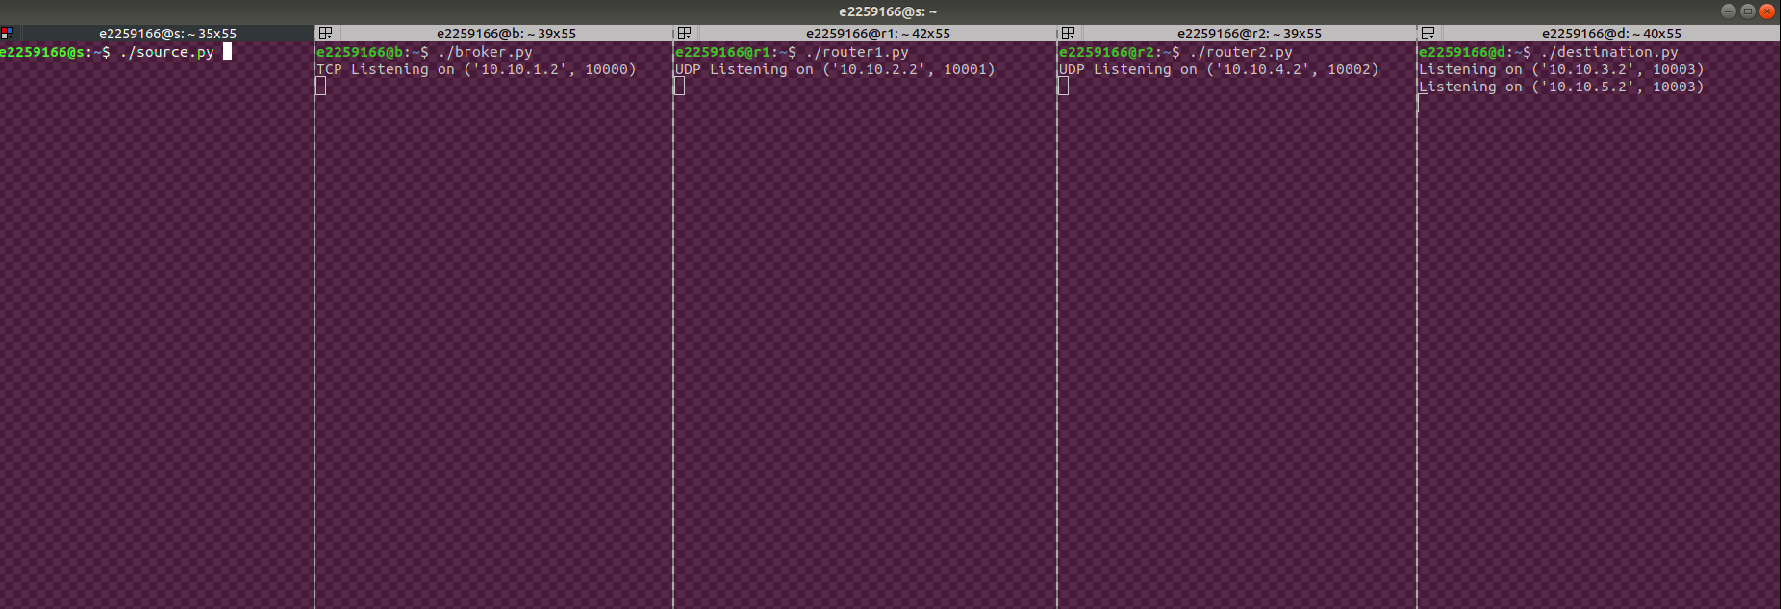
\includegraphics[scale=0.14]{start-up.png}
    \caption{Start Up vision for execution}
\end{figure}


\begin{figure}
    \centering
    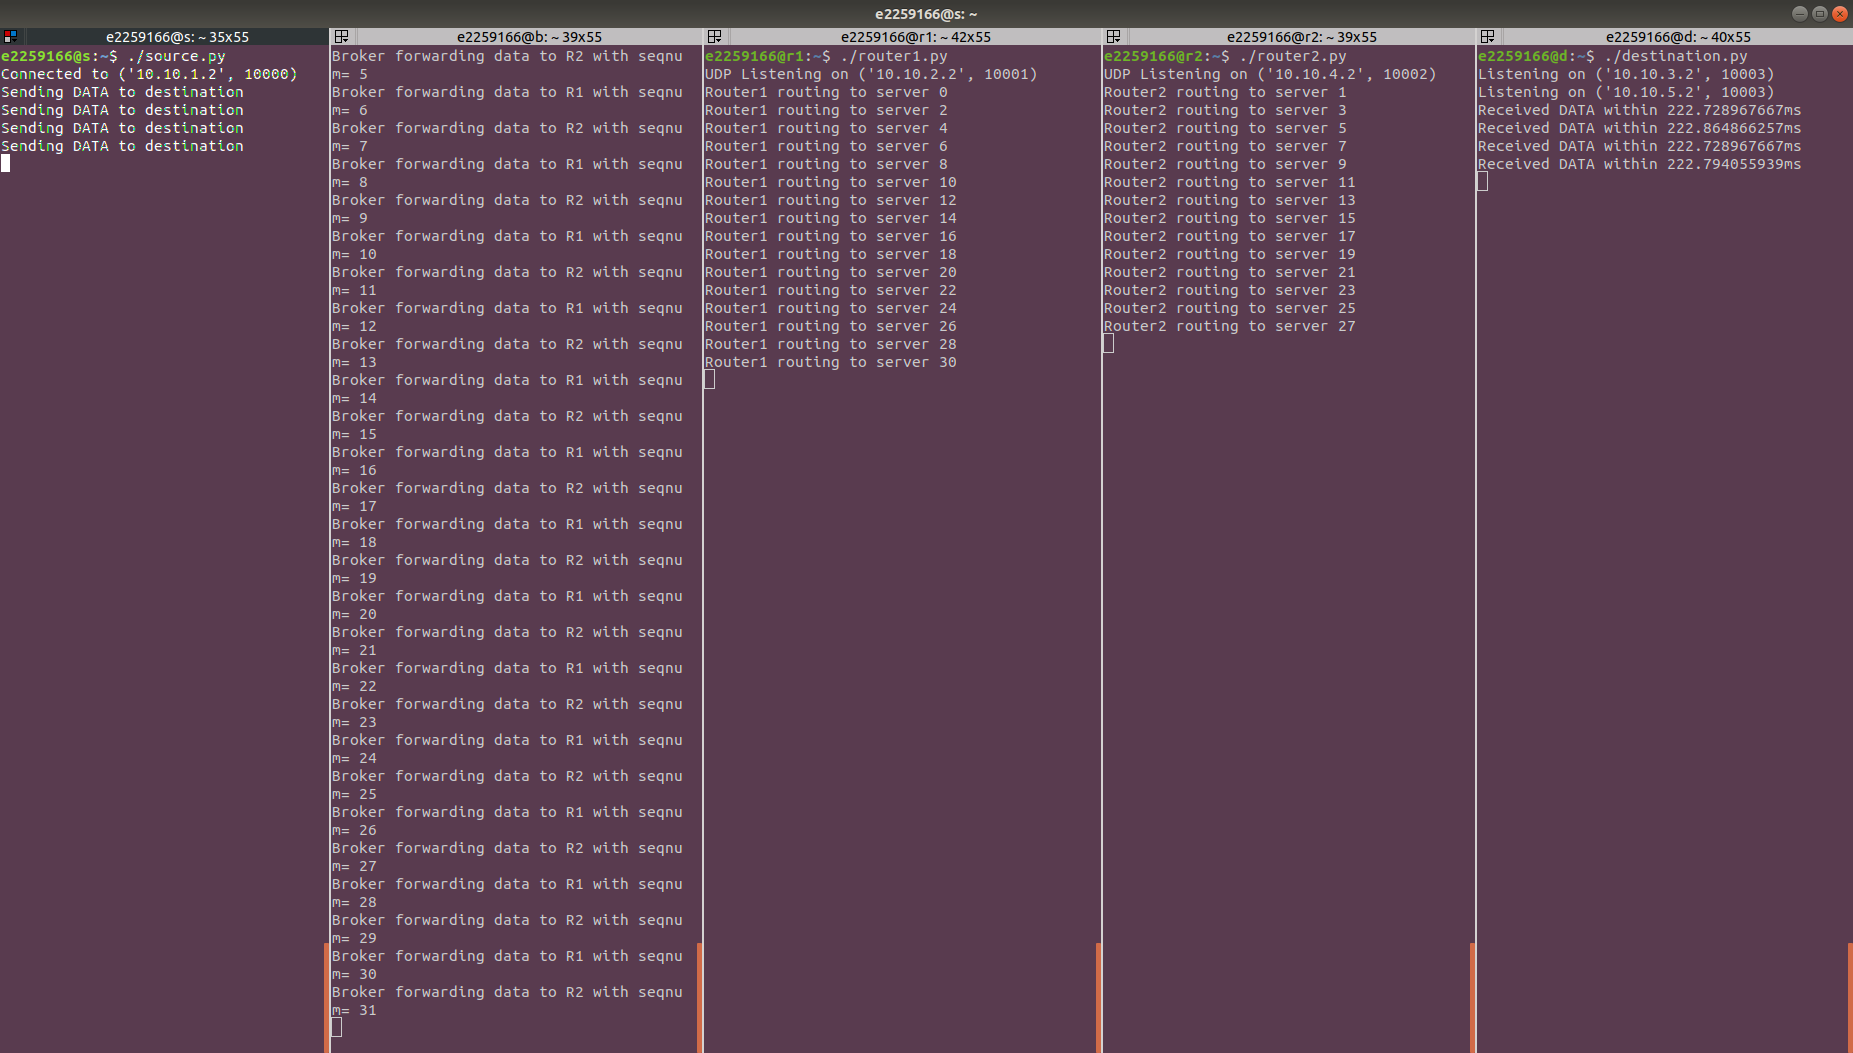
\includegraphics[scale=0.14]{halfway_execution.png}
    \caption{Halfway execution vision}
\end{figure}

Figure 1 shows a screenshot of an example start-up vision for the process and Figure 2 shows a screenshot of an example halfway execution vision of the process. 

\section{Methodology and Motivation}
\subsection{Methodology}
By using "struct" and "time" libraries of Python, time information is added into packets to calculate end to end delay. \\
"threading" and "socket" libraries of Python are used to implement TCP and UDP at the application level and to create multithreaded structure. 

\subsection{Motivation}
This project was helpful for us to learn and experience topics like socket programming with different transport layer protocols, scripting languages and multithreaded structures. We have learned different terms and tools related with stream, packets, protocols and network delay. We have also practiced how to measure or manipulate them. \\

In addition, we have become familiar with the roles of different nodes in networks such as router, broker, receiver and sender nodes. \\

\section{Experimental Results}
\subsection{Tools Used For Experiments}
\textbf{NTP}:
NTP (Network Time Protocol) is a protocol that is used to synchronize clock of computer systems overpacket-switched networks. We used NTP because sending the data computerclock is in nanoseconds, but in network systems packets are sent probably in microseconds, so the packets are received before its time because of the asynchronization.

\textbf{Netem}:
NetEm is an enhancement of the Linux traffic control facilities that allow to add delay, packet loss, duplication and more other characteristics to packets outgoing from a selected network interface. In our experiments we used this command for emulating the delay loss and other similar properties of our network. To achieve this, we applied various kinds of this command for each network interface of the nodes and with some parameters for the virtual machines we created in GENI. \\

\subsection{Experimental Part}
For this part, we mainly made three experiments and plot the information that we gather from these experiments. Since we were needed to repeat the experiment for a considerable amount of time to get meaningful results, we repeated execution exactly 100 times for each experiment. We have achieved that with the help of the file that we created with a bash script on the implementation phase. That file was containing exactly $102400$ bytes which is equal to $102400 = 1024 * 100$ bytes. With this kind of design, since in source node we were just reading data from file as 1024 bytes, execution was getting repeated 100 times. \\

Main task was to calculate end-to-end delays between source and destination nodes, and as mentioned earlier on this report, to achieve this, destination node was calculating each packet's end-to-end delay upon combining the chunks that construct it, then it was storing it to a container. Since we execute our sending data from source to destination process $100$ times, in that container we get 100 end-to-end delays and after sending process terminates destination node calculates average end-to-end delay with taking the mean of the end-to-end delays in that container. \\

For the experiments, firstly we executed our process for $0$ network emulation delay, then we executed it for $1 +- 5$ normally distributed network emulation delay, afterwards we executed it for $20 +- 5$ normally distributed network emulation delay and finally we executed it for $60 +- 5$ normally distributed network emulation delay. The commands that we used for delete, show and add for each experiments are indicated on the README file. \\

On Figure 3 a screenshot of example usage of netem/tc command in our experiments can be seen. On Figure 4,5,6,7 screenshots of the results for the each experiment can be seen clearly (Average end-to-end delays are shown in the rightmost terminal's last line). \\

\begin{figure}
    \centering
    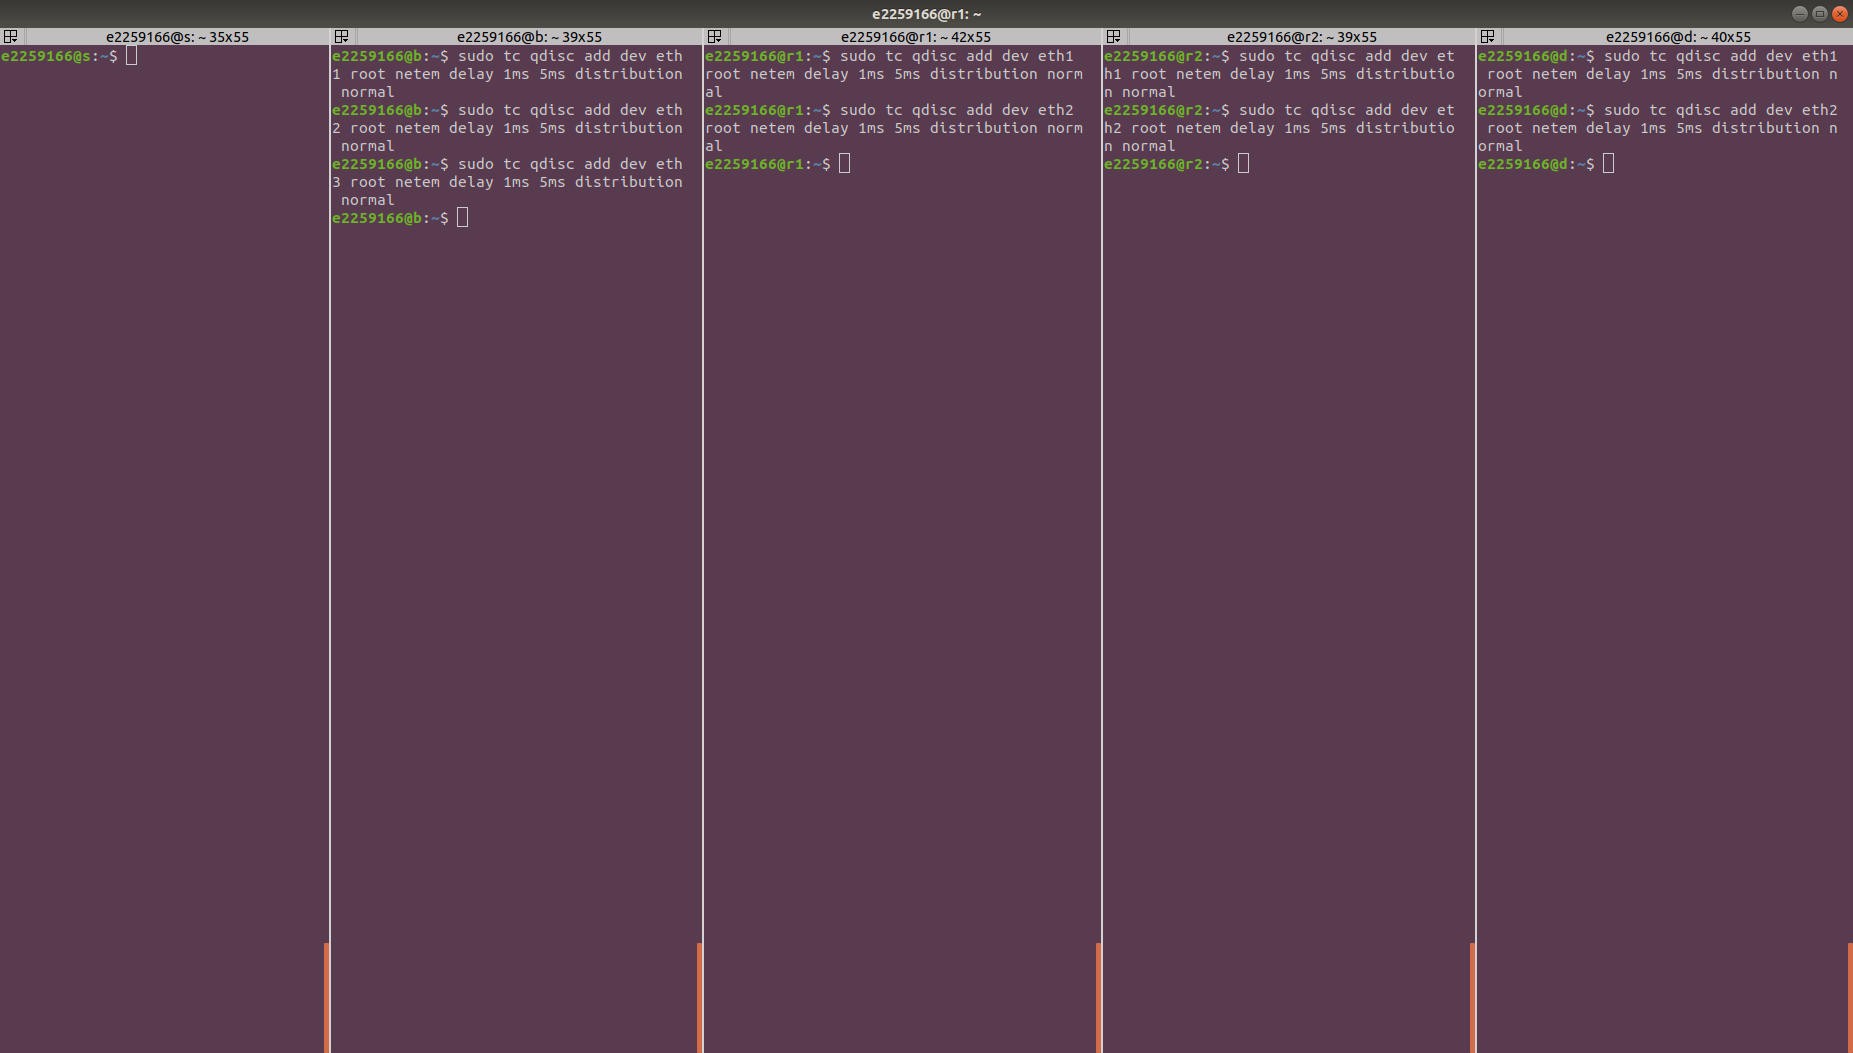
\includegraphics[scale=0.12]{example_tc_usage.png}
    \caption{Example usage of netem/tc command on one our experiments (Shown just for the first experiment)}
\end{figure}

\begin{figure}
    \centering
    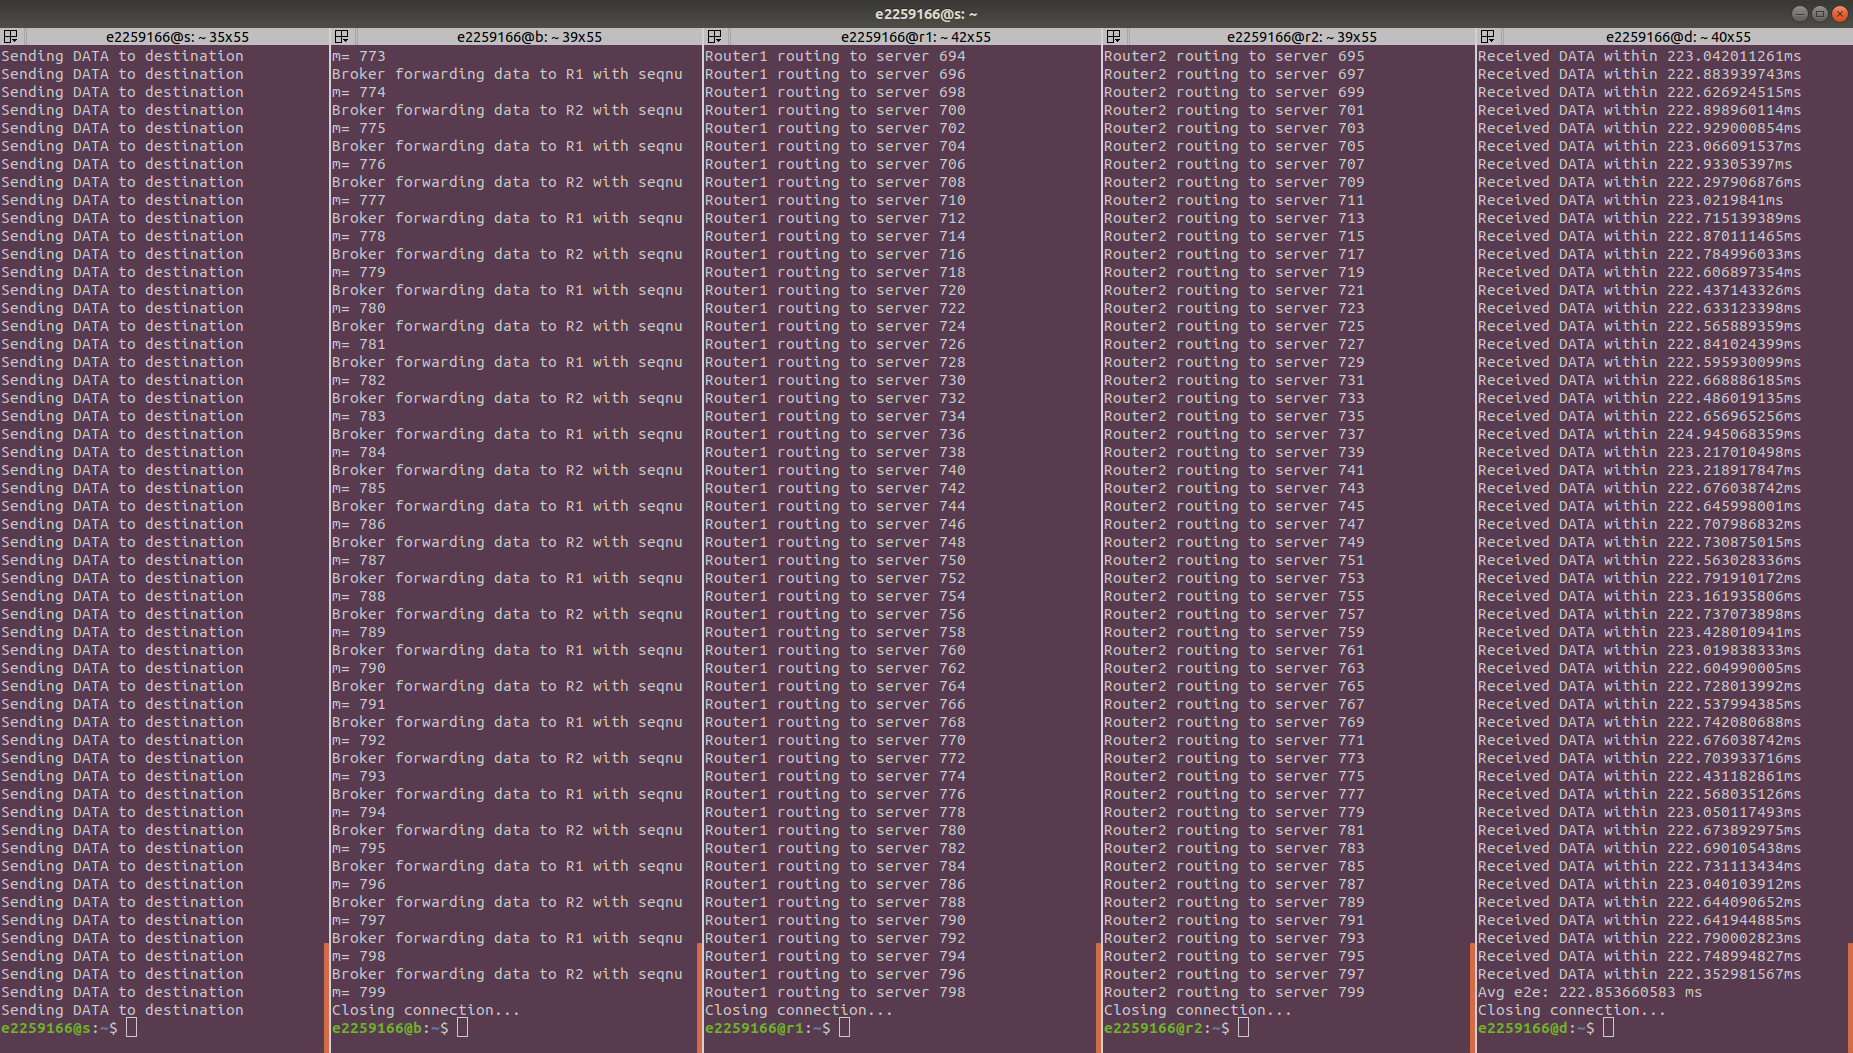
\includegraphics[scale=0.12]{no_delay_result.png}
    \caption{Average end-to-end delay result with No network emulation delay (Shown in rightmost terminal's last line)}
\end{figure}

\begin{figure}
    \centering
    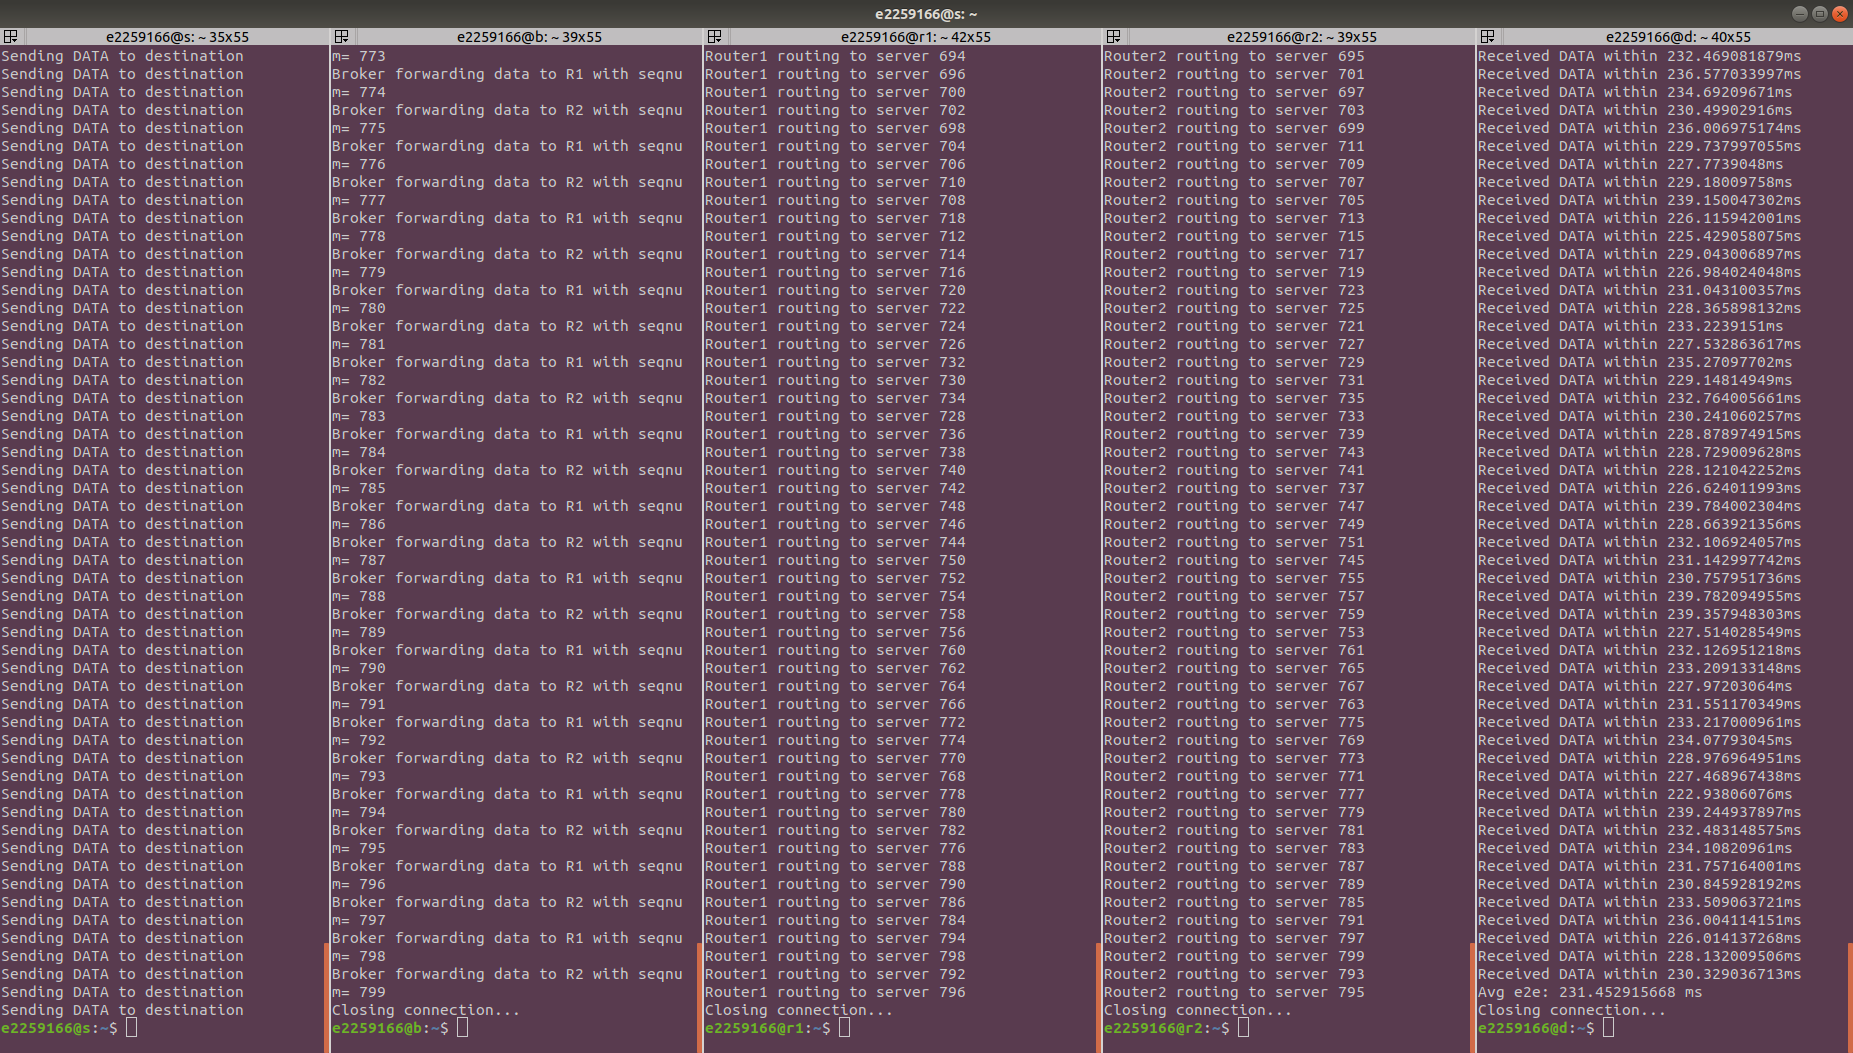
\includegraphics[scale=0.12]{1delay_result.png}
    \caption{Average end-to-end delay result with 1+-5 network emulation delay (Shown in rightmost terminal's last line)}
\end{figure}

\begin{figure}
    \centering
    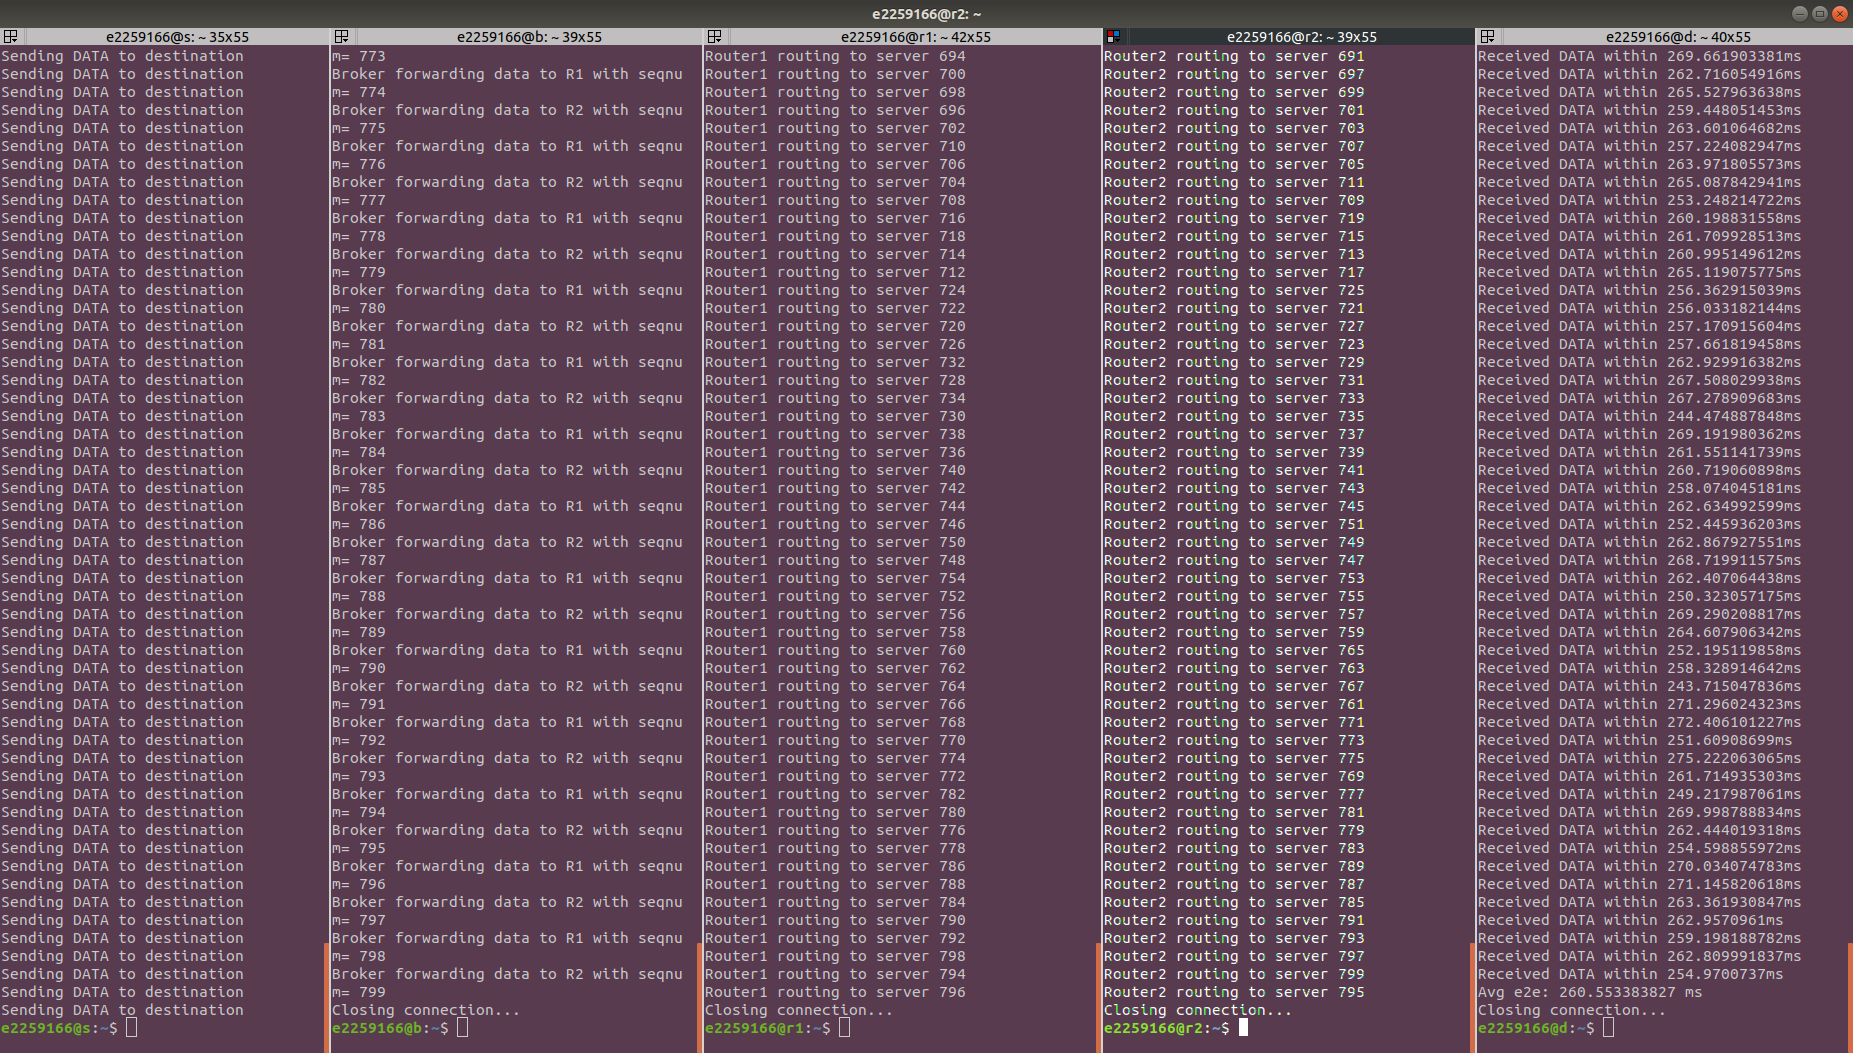
\includegraphics[scale=0.12]{20delay_result.png}
    \caption{Average end-to-end delay result with 20+-5 network emulation delay (Shown in rightmost terminal's last line)}
\end{figure}

\begin{figure}
    \centering
    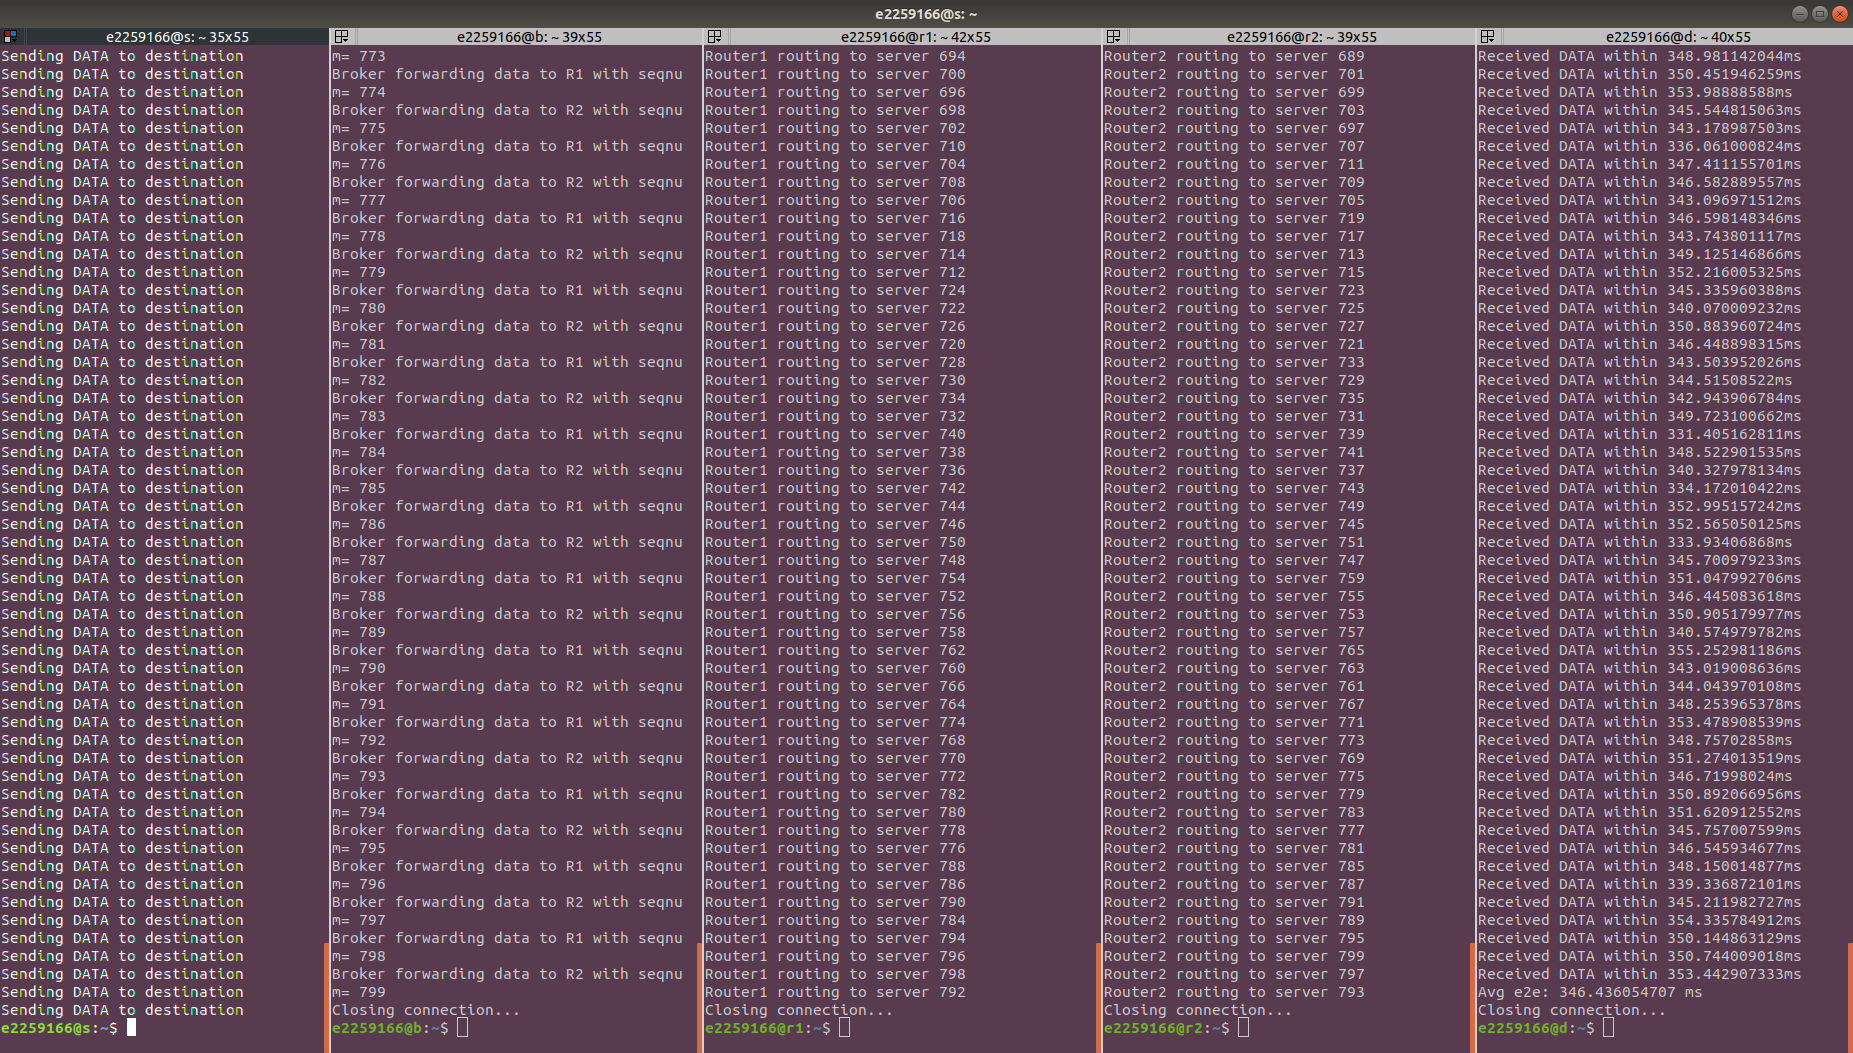
\includegraphics[scale=0.12]{60delay_result.png}
    \caption{Average end-to-end delay result with 60+-5 network emulation delay (Shown in rightmost terminal's last line)}
\end{figure}

To plot graph of end-to-end delay vs network emulation delay with our gatherings from experiments, We also needed to calculate error domains with 95\% Confidence Interval. To achieve this goal, we used following formula for each of the experiments: \\

\begin{align*}
 e &= z \times \frac{(\text{standard deviation for that experiment's delays})}{\sqrt{\text{number of executions}}}  \\\\
   &= 1.960 \times \frac{(\text{standard deviation for that experiment's delays})}{\sqrt{100}} \\
\end{align*}

Where $e$ is error for that experiment, $z$ is the confidence interval variable (for our case, confidence interval = 95\% , so z = 1.960). \\

Upon calculating these errors, we plotted the end-to-end delay vs network emulation delay graph with the help of Octave. Figure 8 shows this graph clearly. \\

For $0$ ms network emulation delay (normal execution of process), we get a result of $222$ ms and for $1$ ms network emulation delay we got a result of $231$ ms. For $20$ ms we get a result of $260$ ms and for $60$ ms network emulation delay we got a result of $346$ ms. First thing we observe is that since we apply network emulation delay for only two links (broker to routers and routers to destination), the delay approximately doubles in the result for the original added delay. The second thing that we see is that resulting graph is a linear fashion increasing graph, namely, as network emulation delay increases end-to-end delay also increases.

\begin{figure}
    \centering
    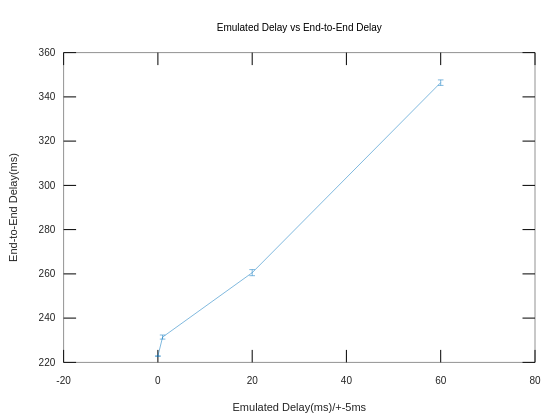
\includegraphics[scale=0.4]{graph.png}
    \caption{Graph of end-to-end delay vs network emulation delay}
\end{figure}

\end{document}
